\subsection{Fight model}\label{chap:fightModel}
We define the \textit{state space} as the set of all possible values the remaining hitpoints of the enemy can have during a fight. For a fight against an enemy with $h$ maximum hitpoints the state space is $\{0,\ldots,h\}$. Each hit corresponds to a transition from one state to another in the state space. The probability of transitioning to state $i$ from state $j$ is called the \textit{transition probability} and is defined as
\begin{align}\label{eq:transitionProbabilities}
    p_{ij} = \Pr{H_k = i \mid H_{k-1} = j}.
\end{align}

Let $H_k$ be the number of hitpoints the enemy has remaining after $k$ hits. A fight can be labeled with a sequence of visited hitpoint states $(H_k)_{k=0}^{n}$. For the sequence to constitute a valid $n$-hit fight we must have $H_n=0$ (fight ends in death) and $h \geq H_k > 0$ for $k<n$ (death does not happen before the last hit). As an example consider a 4-hitpoint enemy that the attacker hits 3 times, first 1, then 0 and finally 3 damage killing the enemy. This fight would be described by the sequence $4,3,3,0$ and corresponds to the highlighted path in the state space diagram in Figure~\ref{fig:stateSpace}.
\begin{figure}[h]
    \centering
    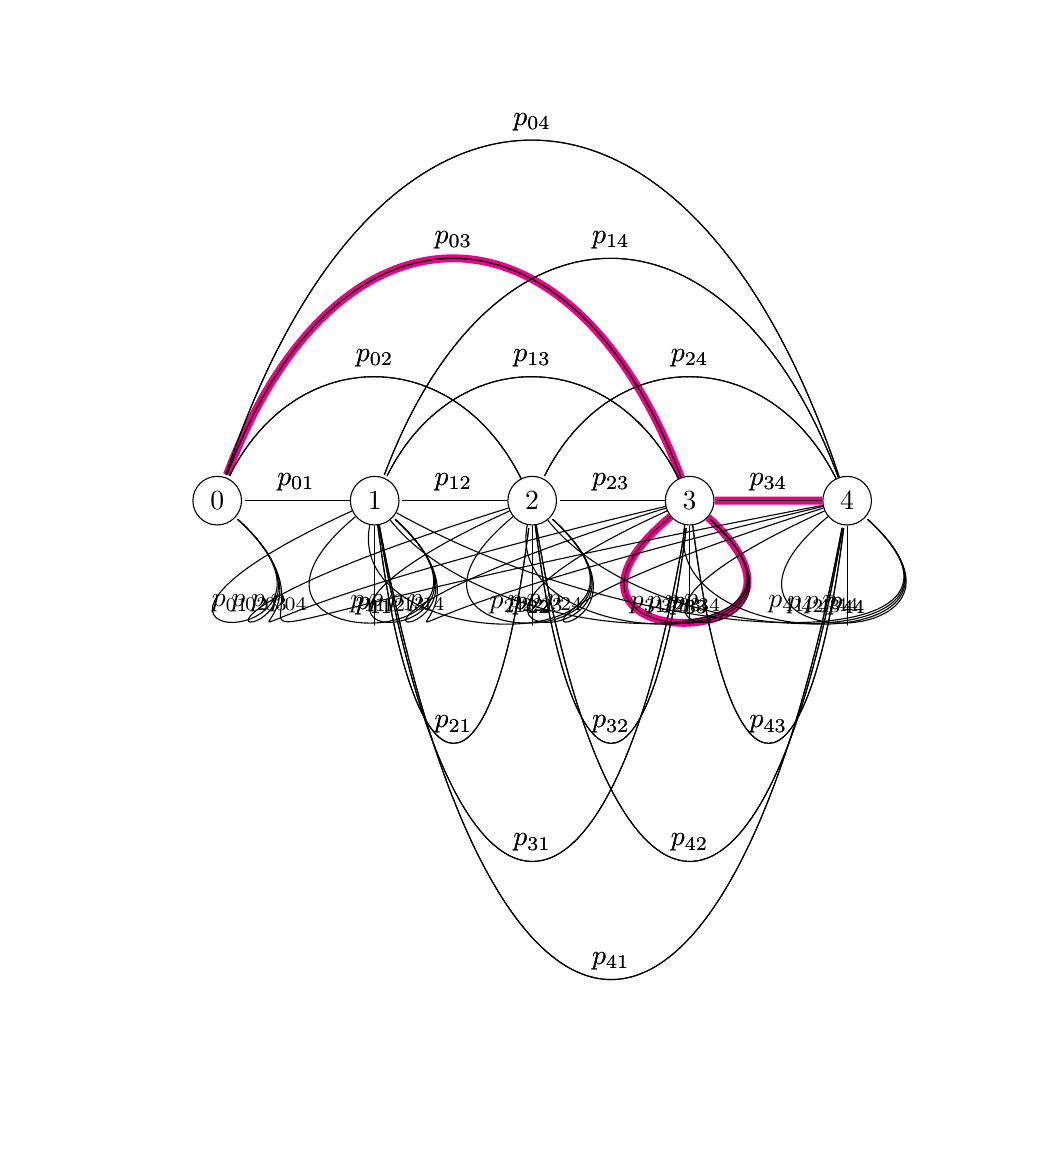
\begin{tikzpicture}[shorten >=1pt,node distance=1cm]
        \tikzstyle{state}=[shape=circle,draw,minimum size=1cm];
        \coordinate (n0);
        \xdef\scale{2}
        \xdef\maxhit{3}
        \foreach \s in {0,1,2,3,4} {
            \node[shape=circle,draw](n\s) at (\scale*\s,0){$\s$};
        }
		\path[draw, color=magenta, line width=1mm] (n4) ..
		controls({(0.75*4+0.25*3)*\scale},{2*(4-3-1)}) and ({(0.25*4+0.75*3)*\scale},{2*(4-3-1)})
		.. (n3) ..
        controls({(3-1.2)*\scale},-2) and ({(3+1.1)*\scale},-2)
		.. (n3) ..
		controls({(0.75*3+0.25*0)*\scale},{2*(3-0-1)}) and ({(0.25*3+0.75*0)*\scale},{2*(3-0-1)})
		.. (n0);
        \foreach \from in {1,2,3,4} {
            \foreach \to in {0,1,2,3,4} {
                \foreach \y [evaluate=\y as \yeval using \from-\to] in {1} {
                \foreach \m [evaluate=\m as \meval using int(\to+\maxhit+1)] in {1} {
                    \ifthenelse{\from>\to \AND \from<\meval \AND \to>0}{
                        \path[draw] (n\from) ..
                        controls({(0.75*\from+0.25*\to)*\scale},{2*(\from-\to-1)}) and ({(0.25*\from+0.75*\to)*\scale},{2*(\from-\to-1)})
                        .. node[above]{$p_{\to\from}$} (n\to);
                    }{}
                    \ifthenelse{\to=0 \AND \from<\meval}{
                        \path[draw] (n\from) ..
                        controls({(0.75*\from+0.25*\to)*\scale},{2*(\from-\to-1)}) and ({(0.25*\from+0.75*\to)*\scale},{2*(\from-\to-1)})
                        .. node[above]{$p_{\to\from}$} (n\to);
                    }{}
                    \ifthenelse{\from=\to}{
                        \path[draw] (n\from) ..
                        controls({(\to-1.2)*\scale},-2) and ({(\to+1.1)*\scale},-2) .. node[above]{$p_{\to\from}$} (n\to);
                    }{}
                }
                }
            }
        }
    \end{tikzpicture}\caption{State space diagram for $m=3$, $h=4$ and no regeneration. The probability of moving to state $i$ from state $j$ is given with the transition probability $p_{ij}$. Only edges for which $p_{ij} > 0$ are shown.}
	\label{fig:stateSpace}
\end{figure}
